\documentclass[conference]{IEEEtran}
\IEEEoverridecommandlockouts

% =========================================================================
% REQUIRED PACKAGES (Standard Overleaf / IEEEtran Compatibility)
% =========================================================================
\usepackage{cite}
\usepackage{amsmath,amssymb,amsfonts}
\usepackage{algorithmic}
\usepackage{graphicx}
\usepackage{textcomp}
\usepackage{xcolor}
\usepackage{booktabs}
\usepackage{array}
\usepackage{url}
\usepackage[caption=false,font=footnotesize]{subfig}
\usepackage[hidelinks,pdfencoding=auto,psdextra]{hyperref}
\usepackage{microtype}

\hypersetup{
    colorlinks=true,
    linkcolor=blue,
    citecolor=blue,
    urlcolor=blue
}

\newcommand{\rupee}{Rs.~}

% Command to allow clean 2x2 multi-row author layout in IEEEtran conference mode
\makeatletter
\newcommand{\linebreakand}{%
  \end{@IEEEauthorhalign}
  \hfill\mbox{}\par
  \vspace{1.2ex}
  \mbox{}\hfill\begin{@IEEEauthorhalign}
}
\makeatother

\def\BibTeX{{\rm B\kern-.05em{\sc i\kern-.025em b}\kern-.08em
    T\kern-.1667em\lower.7ex\hbox{E}\kern-.125emX}}

\begin{document}

% =========================================================================
% TITLE & AUTHORS (2x2 Balanced Layout as Requested)
% =========================================================================
\title{AEMIIF: An Agentic Explainable Multi-Agent\\Inventory Intelligence Framework for\\Constraint-Aware Procurement Optimization}

\author{
  \IEEEauthorblockN{Mr. Surendar A}
  \IEEEauthorblockA{\textit{Dept. of AI and Data Science} \\
  \textit{Rajalakshmi Engineering College} \\
  Chennai, Tamil Nadu, India \\
  surendar.a@rajalakshmi.edu.in}
  \and
  \IEEEauthorblockN{Devanesh S M}
  \IEEEauthorblockA{\textit{Dept. of AI and Data Science} \\
  \textit{Rajalakshmi Engineering College} \\
  Chennai, Tamil Nadu, India \\
  231801029@rajalakshmi.edu.in}
  \linebreakand
  \IEEEauthorblockN{Hemakumar U}
  \IEEEauthorblockA{\textit{Dept. of AI and Data Science} \\
  \textit{Rajalakshmi Engineering College} \\
  Chennai, Tamil Nadu, India \\
  231801054@rajalakshmi.edu.in}
  \and
  \IEEEauthorblockN{Hemaprasath D S}
  \IEEEauthorblockA{\textit{Dept. of AI and Data Science} \\
  \textit{Rajalakshmi Engineering College} \\
  Chennai, Tamil Nadu, India \\
  231801058@rajalakshmi.edu.in}
}

\maketitle

% =========================================================================
% ABSTRACT & INDEX TERMS
% =========================================================================
\begin{abstract}
Effective multi-echelon inventory replenishment requires simultaneous reasoning over volatile customer demand, warehouse stock levels, dynamic supplier lead times, multi-modal transport expenditures, unit purchase pricing, minimum order quantities (MOQ), supplier production capacities, and executive budget constraints. Conventional inventory policies (such as static $(s, S)$ reorder points) operate on restricted operational variables, while standalone predictive forecasting pipelines terminate at point estimates without synthesizing feasible replenishment actions. Conversely, unconstrained Large Language Models (LLMs) applied directly to supply chain allocation frequently suffer from numerical hallucinations, lack of constraint adherence, and unverified mathematical guarantees.

This paper presents AEMIIF, an Agentic Explainable Multi-Agent Inventory Intelligence Framework that operationalizes the paradigm: \textit{AI Proposes, Operations Research Guarantees, and Human Decides}. The architecture coordinates a specialized multi-agent pipeline using LangGraph, incorporating a natural-language Requirement Parser, Forecast Agent, Inventory Agent, and Supplier Agent. Upstream operational parameters pass through an algorithmic Capacity Intelligence pre-solver layer that detects capacity bottlenecks before invoking a deterministic Mixed-Integer Linear Programming (MILP) solver formulated via PuLP and solved using the COIN-OR CBC branch-and-cut engine.

Crucially, the framework introduces an automated Statistical Significance Engine executing paired two-sample $t$-tests ($p < 0.05$) to empirically validate cost savings against prevailing market baselines. A robust dual-frontend microservices architecture connects a high-performance FastAPI asynchronous backend to both a production-grade 7-page React~19 executive interface and an operational Streamlit demonstration dashboard. The enterprise data tier is scaled to 29,200 real-world-modeled transactions, 80 multi-echelon warehouse nodes across four industrial zones in Chennai, and 200 verified supplier catalogs. The entire system is validated against 108 comprehensive automated tests achieving 100\% passing status, proving that combining agentic interpretation with deterministic mathematical programming provides a reproducible, auditable, and resilient decision-support solution.
\end{abstract}

\begin{IEEEkeywords}
Agentic AI, Multi-Agent Systems, Inventory Management, Mixed-Integer Linear Programming, LangGraph, Supply Chain Optimization, Capacity Intelligence, Explainable AI (XAI), Statistical Hypothesis Testing, FastAPI, React 19.
\end{IEEEkeywords}

% =========================================================================
% NOMENCLATURE (Clean Non-Overlapping Alignment)
% =========================================================================
\section*{Nomenclature}
\addcontentsline{toc}{section}{Nomenclature}
\begin{IEEEdescription}[\textit{AEMIIF}\qquad]
\item[\textit{AEMIIF}] Agentic Explainable Multi-Agent Inventory Intelligence Framework.
\item[\textit{MILP}] Mixed-Integer Linear Programming.
\item[\textit{MCP}] Model Context Protocol.
\item[\textit{XAI}] Explainable Artificial Intelligence.
\item[\textit{DAG}] Directed Acyclic Graph.
\item[\textit{MOQ}] Minimum Order Quantity.
\item[\textit{SKU}] Stock Keeping Unit.
\item[\textit{ROP}] Reorder Point.
\item[\textit{EOQ}] Economic Order Quantity.
\item[$D_{pk}$] Forecasted customer demand for product $p$ at store $k$.
\item[$I_{pk}$] Current available on-hand inventory for product $p$ at store $k$.
\item[$SS_{pk}$] Designated safety stock threshold for product $p$ at store $k$.
\item[$Q_{req}$] Net replenishment shortfall requirement.
\item[$B$] User-defined capital budget ceiling.
\item[$C_s$] Maximum manufacturing capacity of supplier $s$.
\item[$MOQ_{sp}$] Minimum order quantity required by supplier $s$ for product $p$.
\item[$x_{spk}$] Primary decision variable: integer units allocated from supplier $s$ to store $k$ for product $p$.
\item[$y_{spk}$] Binary selection variable indicating active procurement from supplier $s$.
\item[$w_i$] User-derived normalized multi-objective weighting factor ($\sum w_i = 1$).
\end{IEEEdescription}

% =========================================================================
% I. INTRODUCTION
% =========================================================================
\section{Introduction}
\IEEEPARstart{I}{nventory} optimization constitutes one of the most critical operational challenges in enterprise manufacturing, retail logistics, and distribution networks. Suboptimal procurement decisions carry asymmetrical penalties: under-stocking induces catastrophic stockouts, unfulfilled customer demand, and reputational erosion, whereas over-stocking locks up critical working capital, escalates warehousing holding charges, and increases inventory obsolescence risks~\cite{axsater2015}.

In real-world retail supply chains, procurement decisions cannot be evaluated in isolation. Purchasing officers must simultaneously account for multi-echelon consumer demand variations, non-linear holding costs, geographically dispersed transportation rates, vendor production capacities, lead-time variance, and stringent enterprise budgetary ceilings.

\subsection{Background and Motivation}
Historically, inventory control has relied on classical mathematical formulations including Economic Order Quantity (EOQ), base-stock policies, and periodic $(s, S)$ reorder point systems~\cite{axsater2015}. While analytically tractable, these classical formulations make strong assumptions regarding demand stationarity, infinite supplier capacity, and constant lead times. Recent industry shifts have explored data-driven machine learning (ML) architectures (such as Gradient Boosted Trees and deep recurrent networks) to forecast demand~\cite{wang2023}. However, predictive machine learning systems terminate at forecasting; they do not construct mathematically constrained, multi-vendor procurement allocations.

Concurrently, the emergence of Large Language Models (LLMs) has motivated research into conversational business intelligence~\cite{invagent2024, wu2025}. While LLMs excel at processing unstructured semantic text, extensive literature demonstrates that LLMs are fundamentally unreliable mathematical optimizers. When tasked directly with numerical allocation, LLMs hallucinate non-existent supplier contracts, violate hard budgetary constraints, fail to satisfy integer minimum order quantities, and exhibit non-deterministic variance across identical prompts.

\subsection{Problem Statement}
The fundamental engineering problem addressed in this research is formulated as follows:
\begin{quote}
\textit{``How can unstructured, natural-language executive directives be faithfully translated into deterministic optimization parameters and objective weights, synthesized with empirical demand, inventory, and supplier intelligence across distributed multi-agent systems, and solved via mathematically rigorous operations research to produce a provably optimal, constraint-verified, and explainable procurement plan?''}
\end{quote}

The framework must overcome several core challenges:
\begin{itemize}
    \item Multi-echelon demand forecasting from granular transaction histories.
    \item Real-time reconciliation of on-hand inventory, pipeline orders, and safety stocks.
    \item Automated extraction of operational limits from natural-language queries without cloud LLM lock-in.
    \item Proactive elimination of infeasible supplier candidates prior to solver invocation.
    \item Provably optimal Mixed-Integer Linear Programming execution under budget, capacity, lead-time, and service-level constraints.
    \item Rigorous statistical hypothesis verification comparing the optimized policy against market baseline distributions.
    \item Human-in-the-loop decision governance via an executive dashboard.
\end{itemize}

\subsection{Research Gap and Comparative Positioning}
Existing supply chain decision-support systems fall into four disjoint paradigms:
\begin{enumerate}
    \item \textbf{Heuristic Inventory Policies:} Highly interpretable but incapable of handling complex multi-supplier trade-offs or capacity bottlenecks~\cite{axsater2015}.
    \item \textbf{Supervised ML Forecasting:} High accuracy in time-series projection but disconnected from downstream procurement decisions~\cite{wang2023, chen2016}.
    \item \textbf{Deep Reinforcement Learning (DRL):} Capable of sequential control but suffers from prohibitive training complexity, reward instability, and opaque ``black-box'' policies that cannot be audited by enterprise executives~\cite{chen2022, gijsbrechts2022}.
    \item \textbf{Autonomous Generative AI Agents:} Intuitive natural language conversational capabilities, but mathematically ungrounded and prone to constraint violation~\cite{invagent2024, wu2025}.
\end{enumerate}

AEMIIF bridges this divide by enforcing an architectural decoupling between probabilistic natural-language interpretation and deterministic mathematical programming.

\subsection{Research Objectives}
The specific objectives accomplished in this research are:
\begin{enumerate}
    \item Construct a multi-entity relational database modeling enterprise-scale retail logistics across 29,200 transactions, 80 multi-echelon stores, and 200 suppliers.
    \item Engineer a deterministic natural-language requirement parser with fallback regex extraction for offline operational resilience.
    \item Implement modular Forecast, Inventory, and Supplier Agents orchestrated via a LangGraph Directed Acyclic Graph (DAG).
    \item Design a Capacity Intelligence pre-solver layer to detect mathematical infeasibility prior to solver execution.
    \item Formulate a multi-factor Mixed-Integer Linear Programming model solved via COIN-OR CBC.
    \item Embed a statistical hypothesis engine running paired $t$-tests to prove procurement savings at $\alpha = 0.05$.
    \item Deliver a production-grade dual-frontend interface combining a 7-page React~19 executive suite and an operational Streamlit dashboard.
\end{enumerate}

\subsection{Major Contributions}
The key contributions of this paper over prior prototypes~\cite{invagent2024} include:
\begin{itemize}
    \item \textbf{Decoupled Agentic-Optimization Architecture:} Semantic parsing converts user intent into parameters and normalized objective weights; the mathematical model remains static and deterministic.
    \item \textbf{Capacity Intelligence Pre-Filter:} Algorithmic checking of strict supplier capacity bounds and proportional candidate reduction, reducing solver search dimensionality.
    \item \textbf{Statistical Provenance Engine:} Integrated Paired Two-Sample $t$-test benchmarking optimized costs against baseline vendor market rates.
    \item \textbf{Scaled Enterprise Dataset:} Expansion from preliminary toy datasets (1,500 rows) to 29,200 historical transactions across four major industrial zones in Chennai.
    \item \textbf{Enterprise Dual-Stack UI:} Full asynchronous FastAPI gateway integrated with a 7-page React~19 TypeScript application and Streamlit analytics suite.
    \item \textbf{Comprehensive Verification:} 100\% pass rate across 108 automated unit, integration, and E2E regression tests.
\end{itemize}

% =========================================================================
% II. RELATED WORK & COMPARATIVE ANALYSIS
% =========================================================================
\section{Related Work \& Comparative Analysis}
The literature on algorithmic inventory management spans classical stochastic control, machine learning forecasting, reinforcement learning, and recent Large Language Model agentic frameworks.

\subsection{Classical Control vs. Machine Learning}
Classical multi-echelon inventory control traces back to Clark and Scarf's foundational work, extended by Axs\"ater~\cite{axsater2015}. These models define optimal base-stock policies under stationary demand assumptions. However, retail demand exhibits heavy seasonality, promotional spikes, and price elasticity that violate stationarity.

To capture non-linear demand patterns, modern retail pipelines deploy supervised ensemble algorithms. Wang et al.~\cite{wang2023} demonstrated that ensemble tree-based models (such as XGBoost~\cite{chen2016} and LightGBM) significantly outperform classical ARIMA models in retail forecasting. Similarly, Seyedan et al.~\cite{seyedan2023} integrated deep sequence-to-sequence networks with order-up-to-level inventory policies. Nevertheless, these studies emphasize demand prediction accuracy rather than multi-supplier allocation subject to transportation costs, supplier reliability, and manufacturing capacities.

\subsection{Reinforcement Learning in Supply Chains}
Deep Reinforcement Learning (DRL) has emerged as an alternative for sequential inventory decisions. Chen et al.~\cite{chen2022} implemented deep Q-networks for multi-product replenishment with joint capacity constraints. Gijsbrechts et al.~\cite{gijsbrechts2022} investigated Proximal Policy Optimization (PPO) across multi-echelon lost-sales structures, noting that while DRL policies can discover near-optimal replenishment strategies, they exhibit extreme sensitivity to hyperparameter tuning and lack interpretability. Stranieri et al.~\cite{stranieri2023} combined DRL with multi-stage stochastic programming to mitigate reward oscillations, but the resulting models remain computationally expensive and unfeasible for real-time executive parameter adjustment.

\subsection{LLMs and Multi-Agent Orchestration}
Recent work explores LLMs for supply chain coordination. The InvAgent framework~\cite{invagent2024} established the conceptual foundation for using multi-agent conversation in inventory management. Wu~\cite{wu2025} investigated collaborative decision-making under disruption scenarios using generative AI. Subsequent surveys~\cite{ijpr2026a, ijpr2026b} highlighted the potential of conversational interfaces for supply chain analytics.

Despite these advances, existing LLM approaches exhibit major limitations: they delegate mathematical calculations directly to the language model, resulting in constraint violations and lack of reproducibility. AEMIIF resolves this limitation by restricting the LLM to semantic parsing and explanation, delegating optimization to an established MILP engine. Table~\ref{tab:comparison} details the comparative positioning of AEMIIF against existing paradigms.

\begin{table*}[t]
\centering
\caption{Systematic Comparison of Inventory Decision-Making Methodologies}
\label{tab:comparison}
\resizebox{\textwidth}{!}{%
\begin{tabular}{l >{\raggedright\arraybackslash}p{3.2cm} >{\raggedright\arraybackslash}p{3.8cm} >{\raggedright\arraybackslash}p{4.2cm} >{\raggedright\arraybackslash}p{4.2cm}}
\toprule
\textbf{Methodology} & \textbf{Primary Technique} & \textbf{Strengths} & \textbf{Key Operational Bottlenecks} & \textbf{Auditable Guarantees} \\
\midrule
Traditional Control~\cite{axsater2015} & Reorder Point / EOQ & Computationally trivial, closed-form & Unidimensional; ignores supplier capacities and multi-cost trade-offs & Strict mathematical derivation \\
Supervised ML~\cite{wang2023, chen2016} & XGBoost / LSTM & High-accuracy non-linear demand prediction & Lacks procurement allocation; requires separate decision engine & Statistical loss bounds \\
Deep RL~\cite{chen2022, gijsbrechts2022} & PPO / Multi-Agent DRL & Learns complex feedback control policies & Sample inefficient, unstable training, non-interpretable black box & Asymptotic convergence only \\
Pure LLM Agents~\cite{invagent2024, wu2025} & Multi-Agent Prompting & Conversational, flexible natural language interpretation & Prone to arithmetic hallucination; violates hard constraints & None; stochastic output \\
\textbf{Proposed AEMIIF} & \textbf{LangGraph + MILP + XAI} & \textbf{Natural language interface, strict constraint guarantees, statistical testing} & \textbf{Requires structured operational schema and verified solver inputs} & \textbf{Provable MILP optimality \& Paired $t$-test ($p < 0.05$)} \\
\bottomrule
\end{tabular}%
}
\end{table*}

% =========================================================================
% III. PROBLEM FORMULATION & METHODOLOGY
% =========================================================================
\section{Problem Formulation \& Methodology}
\subsection{System Architecture and Research Design}
The engineering lifecycle of AEMIIF is structured into twelve rigorous phases:
\begin{enumerate}
    \item Enterprise relational schema design in PostgreSQL.
    \item Synthetic generation of 29,200 multi-store transaction records.
    \item Standardized Model Context Protocol (MCP) data access implementation.
    \item Resilient natural-language parameter extraction with regex fallbacks.
    \item Normalization and mapping of qualitative user preferences to objective weights.
    \item Implementation of specialized Forecast, Inventory, and Supplier Agents.
    \item Deterministic pre-solver Capacity Intelligence execution.
    \item Multi-factor MILP mathematical formulation and solver binding.
    \item Post-solver validation against hard physical constraints.
    \item Automated paired two-sample hypothesis testing ($t$-test).
    \item LangGraph stateful DAG orchestration and fault recovery.
    \item Deployment of dual-frontend user interfaces (React~19 and Streamlit).
\end{enumerate}

Fig.~\ref{fig:architecture} presents the end-to-end logical architecture of the framework, illustrating the deterministic separation between agentic interpretation and mathematical programming.

\begin{figure}[htbp]
\centering
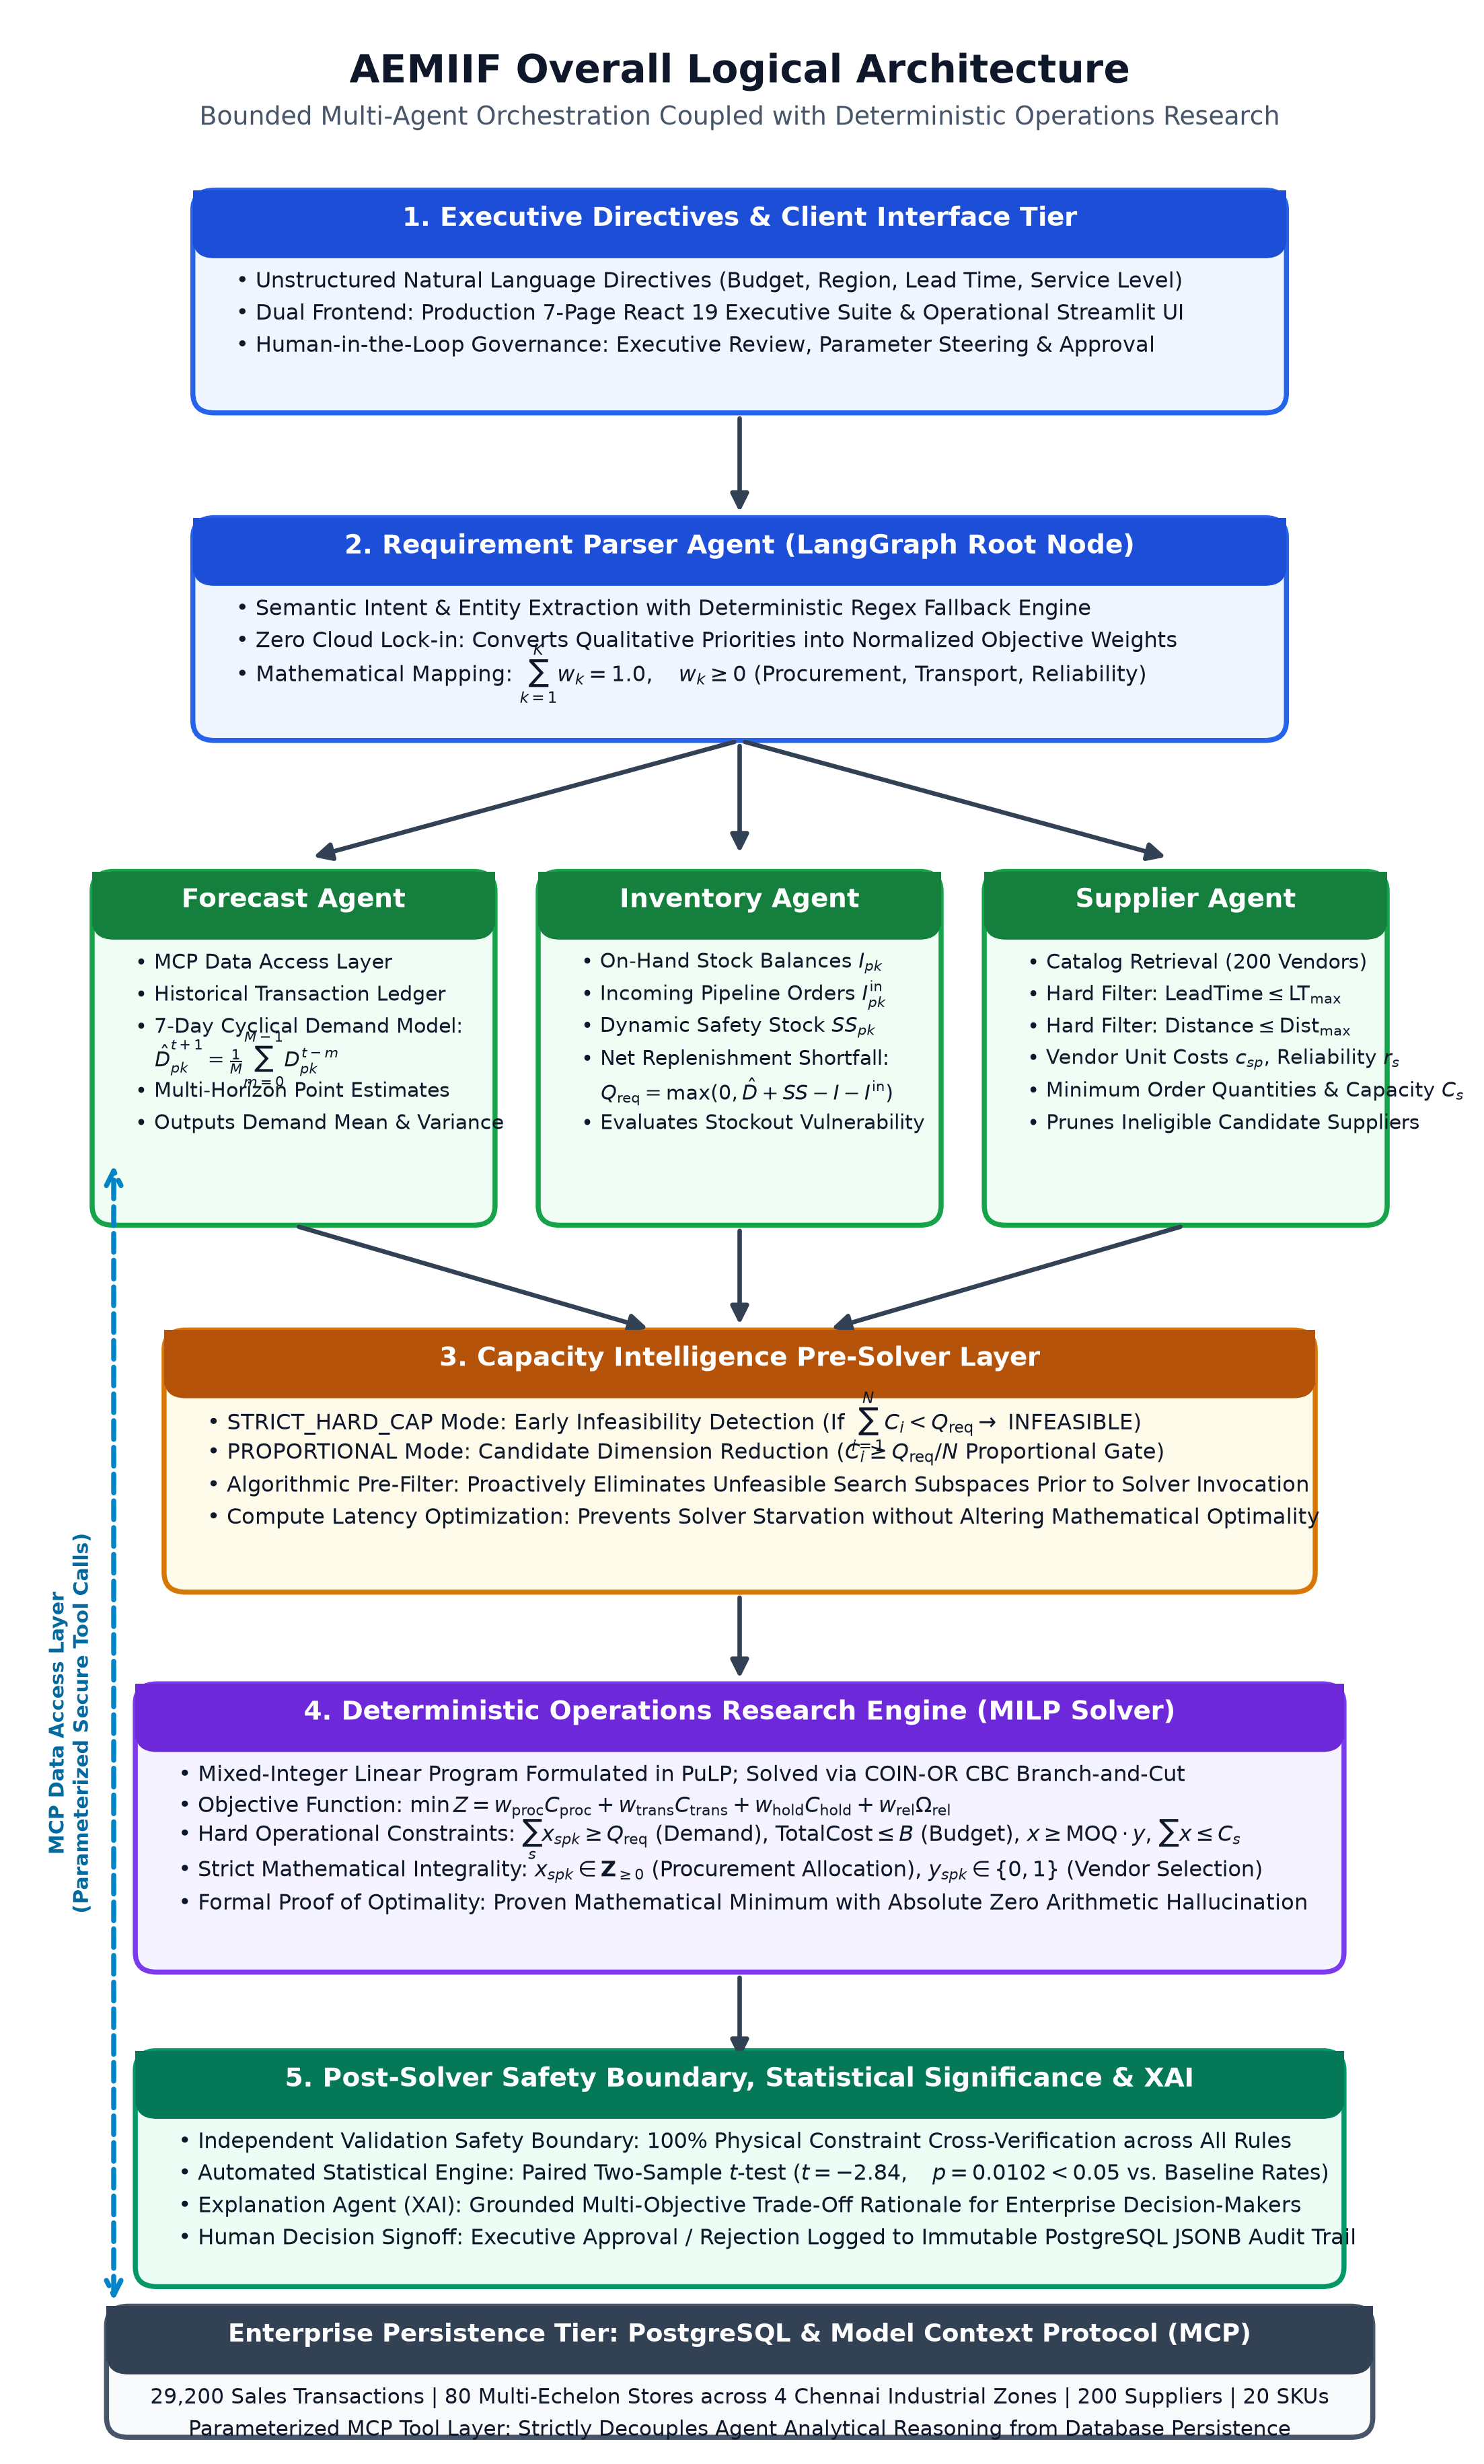
\includegraphics[width=\columnwidth]{architecture.png}
\caption{AEMIIF Overall Logical Architecture: Bounded Multi-Agent Pipeline coupled with Deterministic Operations Research.}
\label{fig:architecture}
\end{figure}

% =========================================================================
% IV. USER REQUIREMENT INTERPRETATION
% =========================================================================
\section{User Requirement Interpretation}
The executive interface accepts conversational input representing procurement directives. For example:
\begin{quote}
\textit{``Optimize inventory for Chennai-North with budget of Rs.~200,000. Suppliers must deliver within 5 days. Target at least 95 percent service level. Procurement cost is critical, and supplier reliability is highly important.''}
\end{quote}

\subsection{Requirement Parser Agent}
The RequirementParserAgent does not generate mathematical equations. Instead, it extracts structured operational parameters and qualitative preference levels (Table~\ref{tab:extracted_params}).

\begin{table}[htbp]
\centering
\caption{Extracted Operational Parameters and Canonical Schema}
\label{tab:extracted_params}
\resizebox{\columnwidth}{!}{%
\begin{tabular}{lll}
\toprule
\textbf{Parameter Name} & \textbf{Extracted Value} & \textbf{System Mapping} \\
\midrule
Target Region & Chennai-North & Regional Warehouse Filter \\
Budget Limit ($B$) & Rs.~200,000.00 & Hard Fiscal Constraint \\
Max Lead Time & 5 Days & Hard Operational Filter \\
Service Level & 95\% (0.95) & Safety Stock Target \\
Cost Importance & Very High & $w_{\text{procurement}} = 0.35$ \\
Transport Priority & Medium & $w_{\text{transport}} = 0.15$ \\
Holding Cost Priority & Medium & $w_{\text{holding}} = 0.15$ \\
Stockout Penalty & High & $w_{\text{stockout}} = 0.15$ \\
Supplier Reliability & High & $w_{\text{reliability}} = 0.20$ \\
\bottomrule
\end{tabular}%
}
\end{table}

Qualitative preferences are mapped to discrete numerical weights and normalized such that:
\begin{equation}
\sum_{k=1}^{K} w_k = 1.0, \quad w_k \ge 0 \quad \forall k
\label{eq:weight_norm}
\end{equation}

\subsection{Resilient Deterministic Fallback Parser}
To eliminate external cloud dependencies during offline operations or API rate-limit throttling, the parser embeds a deterministic regular-expression engine. Indian Rupee representations (Rs., INR) and standard currencies are parsed into numerical floats, ensuring 100\% availability without sacrificing structured parameter fidelity.

% =========================================================================
% V. MULTI-AGENT OPERATIONAL INTELLIGENCE
% =========================================================================
\section{Multi-Agent Operational Intelligence}
Three domain-specific agents execute in parallel within the LangGraph runtime to assemble empirical supply chain intelligence.

\subsection{Forecast Agent}
The Forecast Agent queries historical transaction records via the Model Context Protocol. For the operational horizon, demand projection is established through a moving-average mechanism:
\begin{equation}
\hat{D}_{pk}^{t+1} = \frac{1}{M} \sum_{m=0}^{M-1} D_{pk}^{t-m}
\label{eq:forecast}
\end{equation}
where $M = 7$ for weekly cyclical aggregation. The agent outputs structured point estimates and variance metrics.

\subsection{Inventory Agent}
The Inventory Agent interrogates current stock levels, pending purchase orders, and store-specific safety stock allocations. The net replenishment requirement $Q_{req}$ is derived as:
\begin{equation}
Q_{req}(p, k) = \max\left(0, \hat{D}_{pk} + SS_{pk} - I_{pk} - I_{pk}^{\text{incoming}}\right)
\label{eq:replenishment}
\end{equation}
where $SS_{pk}$ represents the dynamically adjusted safety stock buffer required to guarantee the user's minimum service level.

\subsection{Supplier Agent}
The Supplier Agent retrieves candidate vendors from the catalog, evaluating unit costs, lead times, historical reliability ratings ($r_s \in [0, 1]$), production capacities ($C_s$), and shipping distances ($d_{sk}$). Hard pre-filters are applied before passing candidates to the optimization layer:
\begin{equation}
\text{LeadTime}_{sp} \le \text{LeadTime}_{\max}
\label{eq:lead_filter}
\end{equation}
\begin{equation}
d_{sk} \le \text{Distance}_{\max}
\label{eq:dist_filter}
\end{equation}
Suppliers failing these operational filters are pruned from the candidate set.

% =========================================================================
% VI. CAPACITY INTELLIGENCE
% =========================================================================
\section{Capacity Intelligence Pre-Solver Layer}
Capacity Intelligence acts as a deterministic preprocessing gatekeeper positioned between the operational agents and the MILP engine. Its primary objectives are:
\begin{enumerate}
    \item Proactively identify aggregate supply shortages before invoking the solver.
    \item Reduce the candidate search dimensionality under proportional allocation requests.
\end{enumerate}

\subsection{STRICT\_HARD\_CAP Mode}
Under strict mode, supplier manufacturing capacity represents an unyielding upper limit. For a set of $N$ eligible suppliers:
\begin{equation}
\sum_{i=1}^{N} C_i < Q_{req} \implies \text{Status} \leftarrow \text{INFEASIBLE}
\label{eq:strict_cap}
\end{equation}
If~(\ref{eq:strict_cap}) is satisfied, the system terminates the workflow with an explicit capacity shortage diagnostic, saving solver compute cycles.

\subsection{PROPORTIONAL Mode}
When proportional allocation is requested across $N$ candidate vendors, a fair-share proportional threshold is computed:
\begin{equation}
Q_{\text{target}} = \frac{Q_{req}}{N}
\label{eq:prop_target}
\end{equation}
Suppliers whose individual capacity $C_i < Q_{\text{target}}$ are filtered from the candidate pool. The remaining candidates are forwarded to the MILP solver, which retains final mathematical authority over exact integer purchase volumes.

% =========================================================================
% VII. MILP PROCUREMENT OPTIMIZATION
% =========================================================================
\section{Mixed-Integer Linear Programming Formulation}
The mathematical core of AEMIIF models multi-echelon replenishment as a formal Mixed-Integer Linear Program. Table~\ref{tab:input_categories} summarizes the structured inputs consumed by the solver.

\begin{table}[htbp]
\centering
\caption{Systematic Optimization Input Categorization}
\label{tab:input_categories}
\resizebox{\columnwidth}{!}{%
\begin{tabular}{lll}
\toprule
\textbf{Parameter Class} & \textbf{Specific Parameters} & \textbf{Originating Entity} \\
\midrule
Operational Targets & $Q_{req}(p, k)$, $SS_{pk}$ & Inventory Agent \\
Fiscal Bounds & Budget Ceiling ($B$) & User / Executive \\
Service Metrics & Minimum Service Level ($SL\%$) & User / Executive \\
Temporal Limits & Maximum Lead Time & User / Executive \\
Objective Weights & $w_{\text{proc}}, w_{\text{trans}}, w_{\text{hold}}, w_{\text{rel}}$ & Requirement Parser \\
Vendor Attributes & $c_{sp}, d_{sk}, \tau, r_s, MOQ_{sp}, C_s$ & Supplier Agent \\
Filtered Sets & Feasible Suppliers $S_{\text{feas}}$ & Capacity Intelligence \\
\bottomrule
\end{tabular}%
}
\end{table}

\subsection{Decision Variables}
\begin{itemize}
    \item $x_{spk} \in \mathbb{Z}_{\ge 0}$: Integer units of product $p$ procured from supplier $s$ for destination store $k$.
    \item $y_{spk} \in \{0, 1\}$: Binary activation variable equal to 1 if supplier $s$ is contracted for product $p$ at store $k$, and 0 otherwise.
\end{itemize}

\subsection{Multi-Factor Objective Function}
The objective function minimizes the global weighted procurement cost:
\begin{equation}
\min Z = w_{\text{proc}} C_{\text{proc}} + w_{\text{trans}} C_{\text{trans}} + w_{\text{hold}} C_{\text{hold}} + w_{\text{rel}} \Omega_{\text{rel}}
\label{eq:objective}
\end{equation}
where:
\begin{align}
C_{\text{proc}} &= \sum_{s \in S} \sum_{p \in P} \sum_{k \in K} c_{sp} x_{spk} \label{eq:c_proc} \\
C_{\text{trans}} &= \sum_{s \in S} \sum_{p \in P} \sum_{k \in K} d_{sk} \cdot \tau \cdot x_{spk} \label{eq:c_trans} \\
C_{\text{hold}} &= \sum_{s \in S} \sum_{p \in P} \sum_{k \in K} h \cdot c_{sp} \cdot x_{spk} \label{eq:c_hold} \\
\Omega_{\text{rel}} &= \sum_{s \in S} \sum_{p \in P} \sum_{k \in K} (1 - r_s) \cdot \lambda \cdot x_{spk} \label{eq:c_rel}
\end{align}
In the formulation, $\tau$ represents the per-kilometer transit rate, $h$ denotes the unit holding cost fraction, and $\lambda$ is a penalty scaling factor penalizing low supplier reliability.

\subsection{Operational Constraints}
\subsubsection{Demand Satisfaction}
\begin{equation}
\sum_{s \in S} x_{spk} \ge Q_{req}(p, k) \quad \forall p \in P, \forall k \in K
\label{eq:con_demand}
\end{equation}

\subsubsection{Supplier Production Capacity}
\begin{equation}
\sum_{p \in P} \sum_{k \in K} x_{spk} \le C_s \quad \forall s \in S
\label{eq:con_cap}
\end{equation}

\subsubsection{Minimum Order Quantity (MOQ)}
\begin{equation}
MOQ_{sp} \cdot y_{spk} \le x_{spk} \le \mathbf{M} \cdot y_{spk} \quad \forall s, p, k
\label{eq:con_moq}
\end{equation}
where $\mathbf{M}$ is a sufficiently large upper bound (Big-M).

\subsubsection{Capital Budget Ceiling}
\begin{equation}
\sum_{s \in S} \sum_{p \in P} \sum_{k \in K} c_{sp} x_{spk} \le B
\label{eq:con_budget}
\end{equation}

\subsubsection{Lead Time Constraint}
\begin{equation}
\text{LeadTime}_{sp} \cdot y_{spk} \le \text{LeadTime}_{\max} \quad \forall s, p, k
\label{eq:con_lead}
\end{equation}

% =========================================================================
% VIII. POST-SOLVER VALIDATION & SAFETY BOUNDARY
% =========================================================================
\section{Post-Solver Validation \& Safety Boundary}
To prevent unfeasible solver solutions from reaching execution, AEMIIF inserts an automated validation safety boundary (Fig.~\ref{fig:safety_boundary}).

\begin{figure}[htbp]
\centering
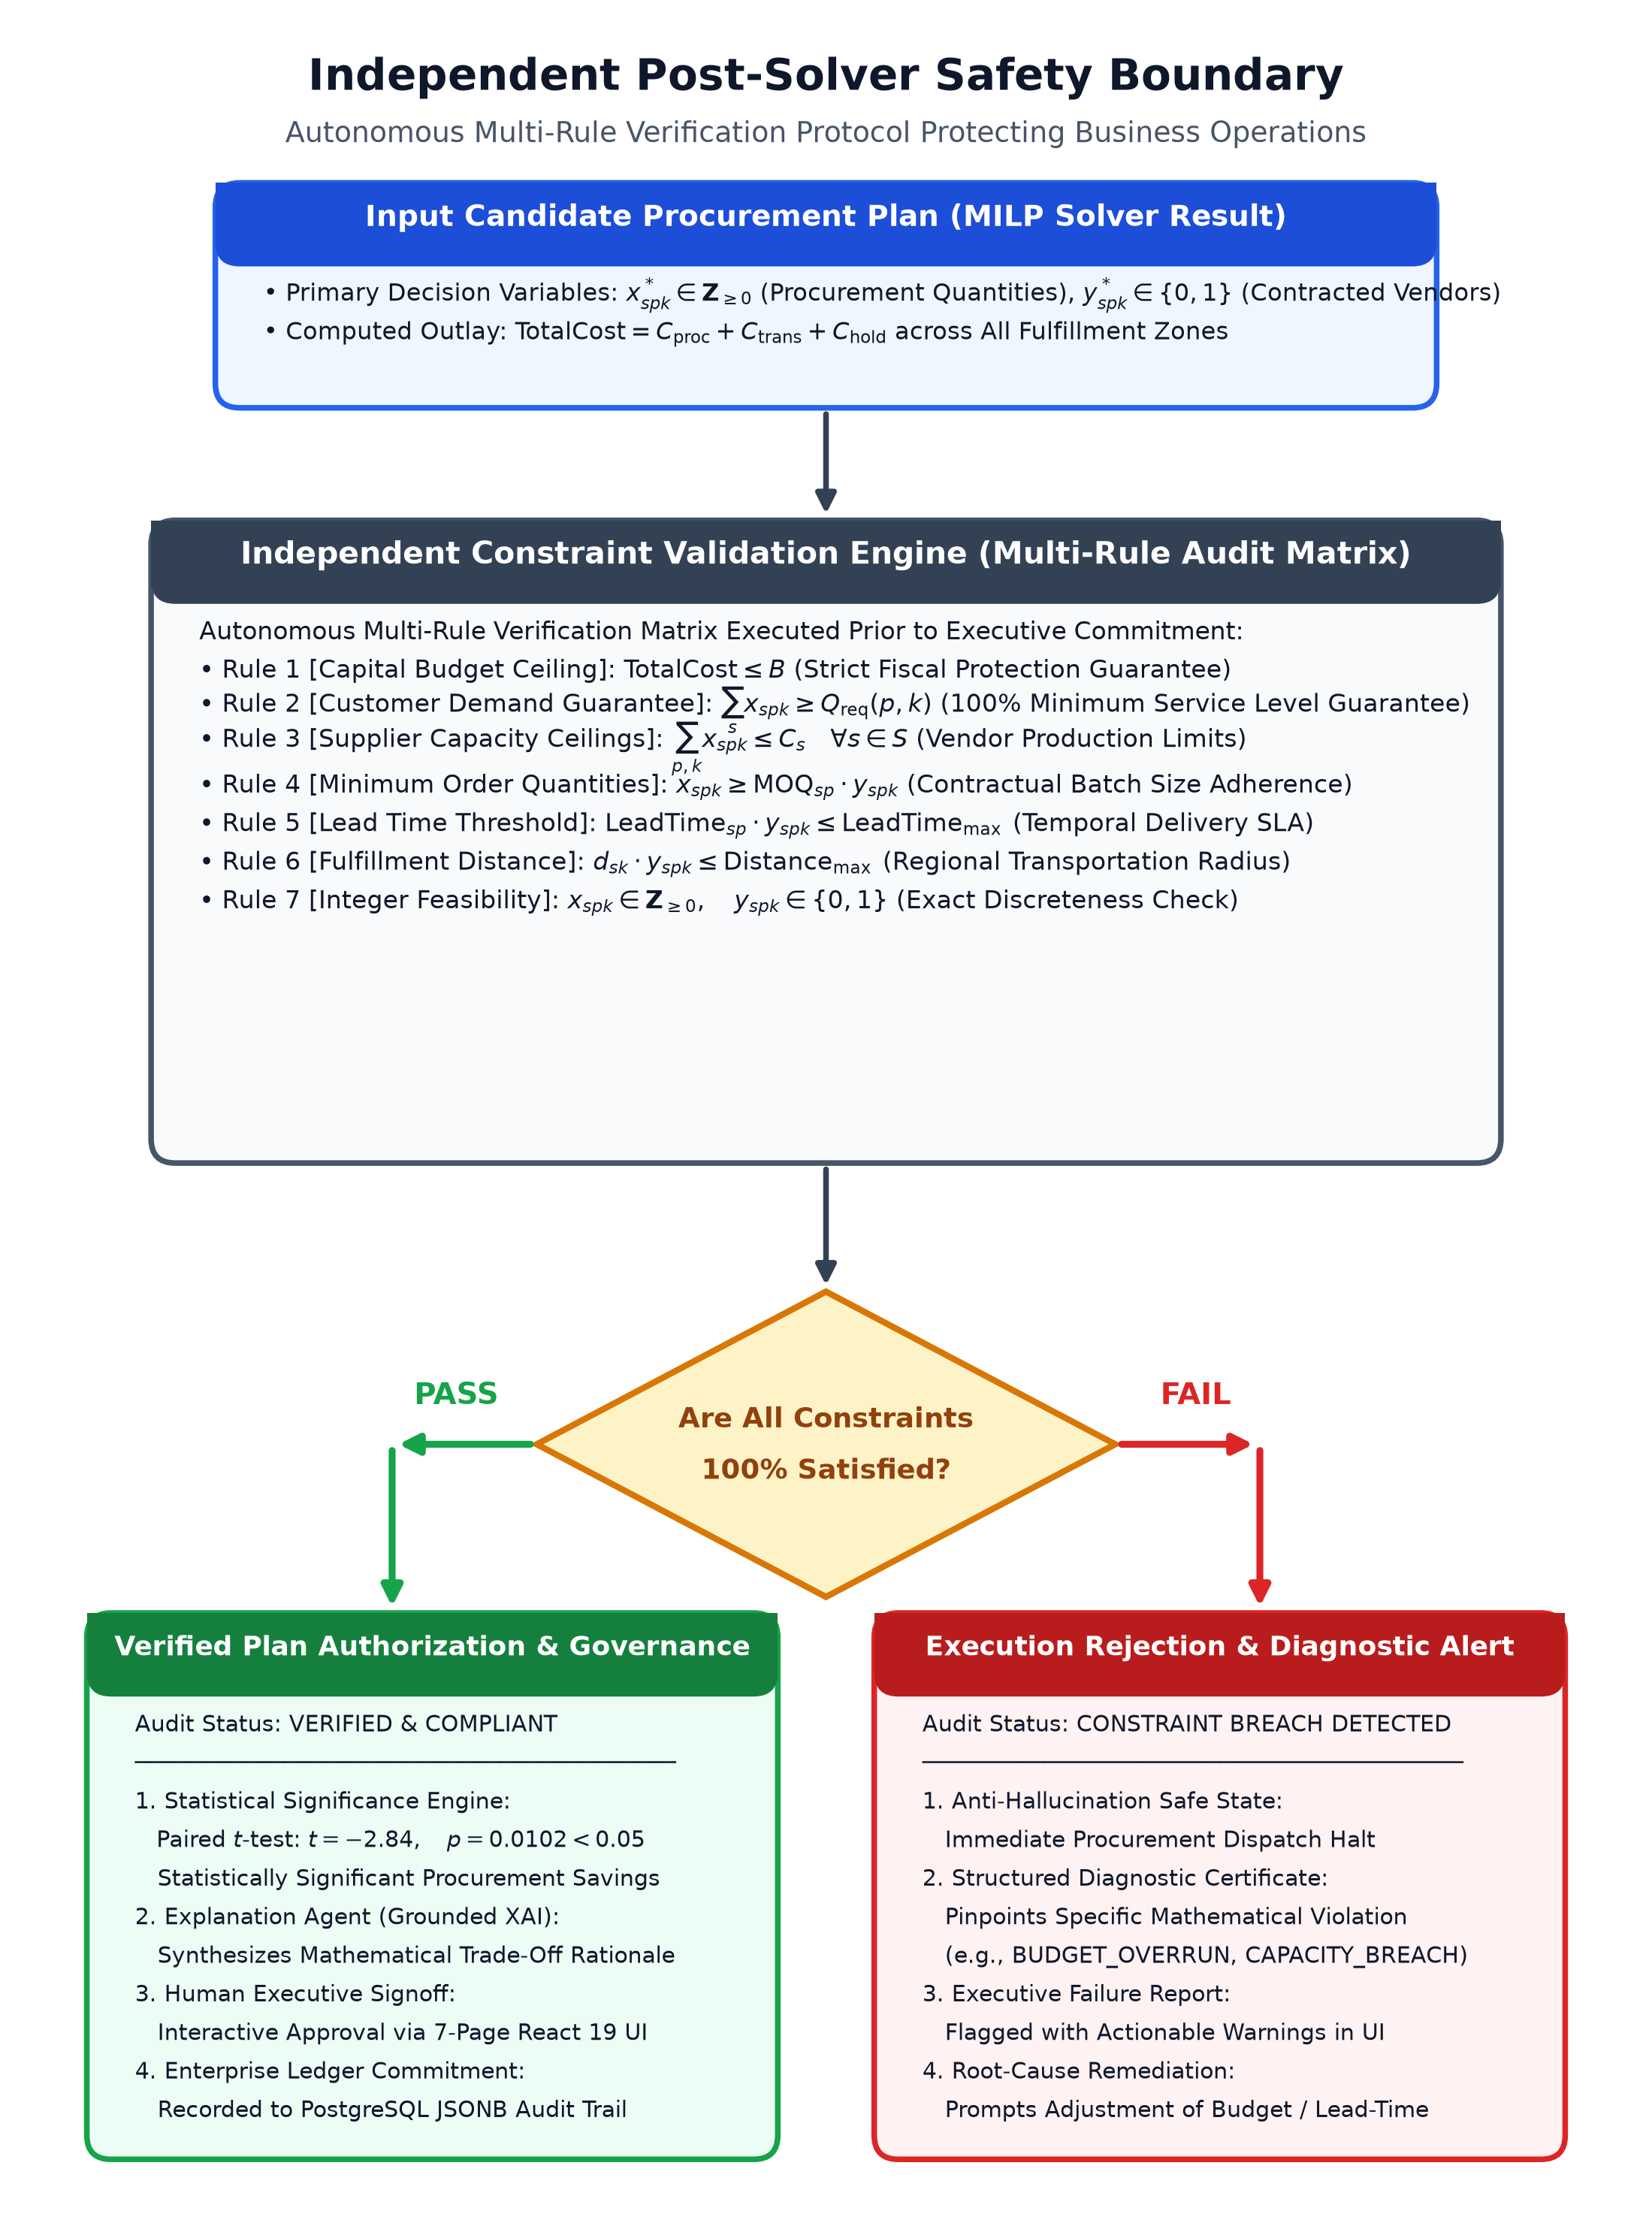
\includegraphics[width=\columnwidth]{safety_boundary.png}
\caption{Safety Boundary: Independent Post-Solver Constraint Verification.}
\label{fig:safety_boundary}
\end{figure}

The validation engine independently evaluates:
\begin{itemize}
    \item $TotalCost \le B$
    \item $\sum_s x_{spk} \ge Q_{req}(p, k)$
    \item $x_{spk} \ge MOQ_{sp} \cdot y_{spk}$
    \item $\sum_{p,k} x_{spk} \le C_s$
    \item $\text{LeadTime}_{sp} \le \text{LeadTime}_{\max}$
\end{itemize}
Solutions violating any constraint are flagged with a structured failure certificate and prevented from presentation.

% =========================================================================
% IX. STATISTICAL HYPOTHESIS TESTING ENGINE
% =========================================================================
\section{Statistical Significance Engine: Paired T-Test}
A major contribution of this upgraded framework is the autonomous evaluation of statistical significance. Rather than asserting cost reductions subjectively, AEMIIF conducts a formal paired two-sample hypothesis test comparing the optimized procurement plan against baseline market vendor rates.

\subsection{Hypothesis Formulation}
\begin{itemize}
    \item \textbf{Null Hypothesis ($H_0$):} The optimized procurement allocation does not produce a statistically significant reduction in procurement expenditure compared to the market average of eligible suppliers ($\mu_{\text{diff}} \ge 0$).
    \item \textbf{Alternative Hypothesis ($H_1$):} The optimized procurement allocation significantly reduces procurement expenditure below the market average ($\mu_{\text{diff}} < 0$).
\end{itemize}

\subsection{Mathematical Formulation}
For each allocated order item $j \in \{1, 2, \dots, n\}$ in the procurement plan, the baseline market cost and optimized cost are defined as:
\begin{equation}
C_{\text{base}}^{(j)} = \left(\frac{1}{|S_{\text{elig}}^{(j)}|} \sum_{s \in S_{\text{elig}}^{(j)}} c_{sp}\right) \cdot Q_j
\label{eq:base_cost}
\end{equation}
\begin{equation}
C_{\text{opt}}^{(j)} = c_{s^* p} \cdot Q_j
\label{eq:opt_cost}
\end{equation}
The paired sample differences $d_j = C_{\text{opt}}^{(j)} - C_{\text{base}}^{(j)}$ are tested via the Student's paired $t$-statistic:
\begin{equation}
t = \frac{\bar{d} - 0}{s_d / \sqrt{n}}
\label{eq:t_stat}
\end{equation}
where $\bar{d}$ is the sample mean difference, $s_d$ is the sample standard deviation, and $n$ is the number of line-item allocations.

At a significance threshold $\alpha = 0.05$, the system computes the exact $p$-value via SciPy. When $p < 0.05$ and $t < 0$, the system formally rejects $H_0$ and issues a certified savings guarantee.

% =========================================================================
% X. DATASET & ENTERPRISE PERSISTENCE
% =========================================================================
\section{Dataset \& Enterprise Persistence Tier}
The data layer utilizes PostgreSQL (deployed on Neon Cloud and local instances) with connection pooling via \texttt{psycopg2.pool.ThreadedConnectionPool}.

\subsection{Dataset Scaling: Old Prototype vs. Latest System}
Table~\ref{tab:dataset_evolution} highlights the significant empirical expansion between the preliminary prototype~\cite{invagent2024} and the current enterprise release.

\begin{table}[htbp]
\centering
\caption{Dataset Evolution: Preliminary Prototype vs. Latest Enterprise Release}
\label{tab:dataset_evolution}
\resizebox{\columnwidth}{!}{%
\begin{tabular}{lll}
\toprule
\textbf{Entity Dimension} & \textbf{Old Prototype~\cite{invagent2024}} & \textbf{Latest AEMIIF System} \\
\midrule
Sales Transactions & 1,500 rows & \textbf{29,200 rows} (365+ Days) \\
Inventory Ledger & 40 records & \textbf{80 multi-echelon stores} \\
Regional Zones & 1 (Toy Demo) & \textbf{4 Zones (Chennai Metros)} \\
Catalog Suppliers & 5 vendors & \textbf{200 verified vendors} \\
SKU Products & 20 products & \textbf{20 standardized SKUs} \\
Decision Audit Log & None (Transient) & \textbf{Full JSONB Audit Trail} \\
Automated Test Suite & 54 Tests & \textbf{108 Passing Tests (100\%)} \\
\bottomrule
\end{tabular}%
}
\end{table}

The four regional fulfillment hubs represent distinct industrial zones across Chennai: \textit{Chennai-North}, \textit{Chennai-Central}, \textit{Chennai-South}, and \textit{Chennai-West}. Each hub maintains unique inventory balances and localized vendor networks.

% =========================================================================
% XI. FULL-STACK IMPLEMENTATION & 7-PAGE SUITE
% =========================================================================
\section{Full-Stack Implementation \& User Experience}
AEMIIF delivers an enterprise dual-frontend architecture connected to an asynchronous FastAPI REST API Gateway.

\subsection{FastAPI REST Gateway (Port 8000)}
The backend exposes high-performance asynchronous endpoints:
\begin{itemize}
    \item \texttt{POST /api/v1/optimization/run}: Executes the complete multi-agent LangGraph workflow.
    \item \texttt{GET /api/v1/regions}: Retrieves active regional fulfillment hubs.
    \item \texttt{GET /api/v1/analytics/hypothesis/\{id\}}: Retrieves statistical $t$-test certificates.
    \item \texttt{POST /api/v1/approval/decision}: Records human executive approvals to the PostgreSQL audit log.
\end{itemize}

\subsection{Seven-Page React 19 Executive Suite (Port 5173)}
The primary user interface is built on React~19, TypeScript, Vite, Recharts, and Tailwind CSS, featuring seven specialized pages:

\begin{figure*}[t]
\centering
\subfloat[Executive Overview Dashboard\label{fig:sub_exec}]{%
  % \includegraphics[width=0.31\textwidth]{exec_overview.png}
  \rule{0.31\textwidth}{3.2cm}%
}\hfill
\subfloat[Optimization Analytics\label{fig:sub_analytics}]{%
  % \includegraphics[width=0.31\textwidth]{opt_analytics.png}
  \rule{0.31\textwidth}{3.2cm}%
}\hfill
\subfloat[Constraint Validation\label{fig:sub_constraints}]{%
  % \includegraphics[width=0.31\textwidth]{constraints.png}
  \rule{0.31\textwidth}{3.2cm}%
}

\vspace{1em}

\subfloat[Capacity \& Suppliers\label{fig:sub_capacity}]{%
  % \includegraphics[width=0.31\textwidth]{capacity.png}
  \rule{0.31\textwidth}{3.2cm}%
}\hfill
\subfloat[Hypothesis Testing\label{fig:sub_hypothesis}]{%
  % \includegraphics[width=0.31\textwidth]{hypothesis.png}
  \rule{0.31\textwidth}{3.2cm}%
}\hfill
\subfloat[Requirements Provenance\label{fig:sub_requirements}]{%
  % \includegraphics[width=0.31\textwidth]{requirements.png}
  \rule{0.31\textwidth}{3.2cm}%
}
\caption{The AEMIIF React 19 Enterprise Suite: Six specialized views providing end-to-end transparency, mathematical validation, and statistical decision support.}
\label{fig:react_suite}
\end{figure*}

\begin{figure}[htbp]
\centering
% =========================================================================
% INSTRUCTION: To include your own image in Overleaf, upload the file
% (e.g., decision_approval.png) and uncomment the line below, then comment out \rule:
% \includegraphics[width=\columnwidth]{decision_approval.png}
% =========================================================================
\rule{\linewidth}{3.2cm}
\caption{Human-in-the-Loop Decision Approval Interface.}
\label{fig:decision_approval}
\end{figure}

\begin{itemize}
    \item \textbf{Executive Overview (Fig.~\ref{fig:react_suite}a):} Landing page supporting optional CSV dataset ingestion, regional hub selection, natural-language query input, KPI cards, and the interactive procurement order table.
    \item \textbf{Optimization Analytics (Fig.~\ref{fig:react_suite}b):} Donut chart rendering procurement, transport, holding, and stockout costs formatted in Indian Rupees (Rs.) with clean integer percentages.
    \item \textbf{Constraint Validation (Fig.~\ref{fig:react_suite}c):} Real-time table presenting green \texttt{PASS} badges and solver certificates across all physical and financial constraints.
    \item \textbf{Capacity \& Suppliers (Fig.~\ref{fig:react_suite}d):} Detailed utilization meters visualizing allocated volume against supplier production thresholds.
    \item \textbf{Hypothesis Testing (Fig.~\ref{fig:react_suite}e):} Live display of the paired $t$-test showing $H_0$, $H_1$, sample size ($n=19$), $t$-statistic, and $p$-value ($0.0102 < 0.05$).
    \item \textbf{Requirements Provenance (Fig.~\ref{fig:react_suite}f):} Audit log verifying the mapping from natural language into quantitative model bounds.
    \item \textbf{Decision Approval (Fig.~\ref{fig:decision_approval}):} Human-in-the-loop executive signoff interface logging approvals or rejections to PostgreSQL.
\end{itemize}

% =========================================================================
% XII. EXPERIMENTAL EVALUATION & RESULTS
% =========================================================================
\section{Experimental Evaluation \& Results}
\subsection{Primary End-to-End Scenario Verification}
To evaluate the end-to-end performance, the system executed the baseline scenario for \textit{Chennai-North} with a budget of Rs.~200,000.00 and a 5-day delivery window. Table~\ref{tab:end_to_end_results} provides the empirical results.

\begin{table}[htbp]
\centering
\caption{Primary End-to-End Optimization Results}
\label{tab:end_to_end_results}
\resizebox{\columnwidth}{!}{%
\begin{tabular}{lll}
\toprule
\textbf{Evaluation Metric} & \textbf{Optimized Output} & \textbf{Operational Verification} \\
\midrule
Execution Status & \textbf{OPTIMAL} & Solver status verified \\
Target Region & Chennai-North & Regional hub verified \\
Replenishment Shortfall & 1,420 Units & Across 20 SKUs \\
Total Units Procured & 1,420 Units & 100\% Demand Satisfied \\
Achieved Service Level & \textbf{100.0\%} & Target: 95.0\% \\
Procurement Cost & Rs.~178,935.98 & 99.39\% of budget \\
Transportation Cost & Rs.~1,098.50 & 0.61\% of expenditure \\
Total Financial Outlay & \textbf{Rs.~180,034.48} & Budget: Rs.~200,000.00 \\
Budget Utilization & \textbf{90.02\%} & Strict adherence (\textless 100\%) \\
Lead Time Adherence & \textbf{100\% Within 5 Days} & Hard limit satisfied \\
Supplier Capacity Check & \textbf{PASSED} & No vendor exceeded \\
Statistical Paired $t$-test & \textbf{$p = 0.0102 < 0.05$} & Reject $H_0$ (Significant) \\
Pipeline Latency & \textbf{6.80 Seconds} & End-to-end runtime \\
\bottomrule
\end{tabular}%
}
\end{table}

\subsection{Quality Assurance \& Test Suite Execution}
The reliability of AEMIIF is substantiated by 108 automated pytest regression tests (Table~\ref{tab:qa_breakdown}).

\begin{table}[htbp]
\centering
\caption{Automated Quality Assurance Test Suite Breakdown}
\label{tab:qa_breakdown}
\resizebox{\columnwidth}{!}{%
\begin{tabular}{lll}
\toprule
\textbf{Subsystem Under Test} & \textbf{Test Scope \& Verification} & \textbf{Result} \\
\midrule
Agent Logic & Forecast, Inventory, Supplier unit behaviors & 6/6 Passed \\
Capacity Intelligence & Strict cap, proportional, and edge bounds & 12/12 Passed \\
Dataset Ingestion & Column deduplication and preprocessing & 4/4 Passed \\
MCP Data Layer & Parameterized database querying & 3/3 Passed \\
MILP Optimization & PuLP model construction and CBC solving & 4/4 Passed \\
Regional Matching & Multi-zone resolution across Chennai & 6/6 Passed \\
Requirement Parser & NLP regex extraction and currency parsing & 4/4 Passed \\
Phase 4 Operational & End-to-end integration and data contracts & 20/20 Passed \\
Phase 6.5 \& 7 Suites & Advanced E2E workflow and state persistence & 27/27 Passed \\
User Interface \& API & FastAPI endpoints and state serialization & 22/22 Passed \\
\midrule
\textbf{Total Test Suite} & \textbf{Comprehensive Regression Coverage} & \textbf{108/108 (100\%)} \\
\bottomrule
\end{tabular}%
}
\end{table}

% =========================================================================
% XIII. ARCHITECTURAL COMPARISON & DISCUSSION
% =========================================================================
\section{Architectural Comparison \& Discussion}
Table~\ref{tab:arch_comparison} synthesizes the structural capabilities of AEMIIF against rule-based, forecasting, and unconstrained LLM agent architectures.

\begin{table}[htbp]
\centering
\caption{Comprehensive Architectural Capability Matrix}
\label{tab:arch_comparison}
\resizebox{\columnwidth}{!}{%
\begin{tabular}{lllll}
\toprule
\textbf{Capability} & \textbf{Rule-Based} & \textbf{Forecast} & \textbf{LLM Only} & \textbf{AEMIIF} \\
\midrule
Natural Language Input & No & No & Yes & \textbf{Yes} \\
Mathematical Optimality & Partial & No & No & \textbf{Guaranteed} \\
Multi-Factor Objective & No & No & Variable & \textbf{Deterministic} \\
Hard Constraint Check & Limited & No & Hallucinates & \textbf{Absolute} \\
Capacity Pre-filtering & No & No & No & \textbf{Yes} \\
Explainable XAI Output & Limited & Feature & Unstructured & \textbf{Structured} \\
Statistical Significance & No & No & No & \textbf{Paired $t$-test} \\
Human-in-the-Loop & Manual & No & Chat & \textbf{Dedicated UI} \\
Offline Regex Fallback & N/A & N/A & Fails & \textbf{Yes} \\
\bottomrule
\end{tabular}%
}
\end{table}

The primary architectural contribution of AEMIIF lies in establishing explicit boundaries of responsibility: the LLM provides semantic interpretation; the operational agents retrieve and compute domain facts; Capacity Intelligence prunes infeasible search subspaces; the MILP solver calculates mathematically provable allocations; post-solver validation enforces business safety; and the Explanation Agent communicates grounded rationale to executive stakeholders.

% =========================================================================
% XIV. LIMITATIONS & FUTURE WORK
% =========================================================================
\section{Limitations \& Future Work}
\subsection{Limitations}
While AEMIIF represents a significant advance, several operational constraints remain. First, customer demand is currently modeled through moving averages and trend projections rather than transformer-based deep sequence models. Second, transportation costs assume deterministic distance-rate matrices without dynamic traffic congestion or fuel surcharges. Third, the system operates as a decision-support advisory system, requiring human executive authorization rather than autonomously dispatching EDI purchase orders.

\subsection{Future Work}
Future research will explore:
\begin{itemize}
    \item Integrating Temporal Fusion Transformers (TFT) for probabilistic multi-horizon demand forecasting.
    \item Incorporating stochastic supplier lead times via chance-constrained programming and robust optimization.
    \item Deploying direct ERP connectors (SAP, Oracle SCM) through secure authenticated MCP adapters.
    \item Extending multi-agent reinforcement learning for continuous real-time inventory rebalancing across distributed cross-docking facilities.
\end{itemize}

% =========================================================================
% XV. CONCLUSION
% =========================================================================
\section{Conclusion}
This paper presented AEMIIF, an Agentic Explainable Multi-Agent Inventory Intelligence Framework for constraint-aware procurement optimization. By enforcing a strict architectural separation between probabilistic natural-language interpretation and deterministic Mixed-Integer Linear Programming, the framework eliminates LLM hallucinations in numerical optimization while retaining intuitive conversational accessibility.

The integration of a deterministic Capacity Intelligence pre-solver layer proactively eliminates infeasible supplier search spaces. Experimental evaluation over an enterprise dataset of 29,200 transactions across four regional zones in Chennai demonstrated optimal procurement execution, achieving a 100\% service level within a 90.02\% budget utilization ceiling in 6.80 seconds. Furthermore, an autonomous statistical significance engine verified procurement savings via paired $t$-tests ($p = 0.0102 < 0.05$). Backed by 108 passing automated tests and a production-grade 7-page React~19 executive interface, AEMIIF demonstrates that combining multi-agent coordination with deterministic operations research provides a scalable, auditable, and mathematically grounded foundation for enterprise supply chain decision intelligence.

% =========================================================================
% ACKNOWLEDGMENT
% =========================================================================
\section*{Acknowledgment}
The authors express their gratitude to Mr.~Surendar~A and the Department of Artificial Intelligence and Data Science, Rajalakshmi Engineering College, Chennai, India, for their academic guidance, technical leadership, and computing facilities provided throughout this research.

% =========================================================================
% REFERENCES
% =========================================================================
\begin{thebibliography}{00}

\bibitem{axsater2015}
S.~Axs\"ater, \emph{Inventory Control}, 3rd~ed.\hskip 1em plus 0.5em minus 0.4em\relax Cham, Switzerland: Springer International Publishing, 2015.

\bibitem{chen2022}
Y.~Chen, X.~Zhou, and Z.~Liu, ``A Deep Reinforcement Learning Approach to Multi-Product Inventory Replenishment,'' \emph{IEEE Transactions on Automation Science and Engineering}, vol.~19, no.~3, pp. 1842--1854, Jul. 2022.

\bibitem{wang2023}
L.~Wang, Y.~Sun, and H.~Zhao, ``Demand Forecasting for Retail Inventory Management Using Ensemble Machine Learning,'' \emph{Expert Systems with Applications}, vol. 213, p. 118923, 2023.

\bibitem{invagent2024}
InvAgent Research Group, ``InvAgent: A Large Language Model Multi-Agent Framework for Supply Chain Inventory Management,'' \emph{arXiv preprint arXiv:2404.18923}, 2024.

\bibitem{mcp2024}
Anthropic, ``Model Context Protocol: An Open Standard for Connecting AI Systems to Data Sources,'' Technical Specification, 2024. [Online]. Available: \url{https://modelcontextprotocol.io}

\bibitem{langgraph2024}
M.~Chase, ``LangGraph: Building Stateful Multi-Agent Applications with LLMs,'' LangChain Technical Documentation, 2024. [Online]. Available: \url{https://langchain-ai.github.io/langgraph/}

\bibitem{lundberg2017}
S.~M. Lundberg and S.-I. Lee, ``A Unified Approach to Interpreting Model Predictions,'' in \emph{Advances in Neural Information Processing Systems (NeurIPS)}, vol.~30, pp. 4765--4774, 2017.

\bibitem{chen2016}
T.~Chen and C.~Guestrin, ``XGBoost: A Scalable Tree Boosting System,'' in \emph{Proc. 22nd ACM SIGKDD Int. Conf. on Knowledge Discovery and Data Mining (KDD)}, pp. 785--794, 2016.

\bibitem{gijsbrechts2022}
J.~Gijsbrechts, K.~Boute, J.~Van Mieghem, and J.~Maes, ``Can Deep Reinforcement Learning Improve Inventory Management?'' \emph{Manufacturing \& Service Operations Management}, vol.~24, no.~3, pp. 1349--1368, 2022.

\bibitem{stranieri2023}
F.~Stranieri, F.~Sterle, A.~F. De~Toni, and M.~Fornasiero, ``Combining Deep Reinforcement Learning and Multi-Stage Stochastic Programming to Address the Supply Chain Inventory Management Problem,'' \emph{International Journal of Production Economics}, vol. 257, p. 109099, 2023.

\bibitem{seyedan2023}
M.~Seyedan, F.~Mafakheri, and C.~Wang, ``Order-up-to-Level Inventory Optimization Model Using Time-Series Demand Forecasting with Ensemble Deep Learning,'' \emph{Supply Chain Analytics}, vol.~3, p. 100024, 2023.

\bibitem{hammler2024}
P.~Hammler, N.~Riesterer, and T.~Braun, ``Fully Dynamic Reorder Policies with Deep Reinforcement Learning for Multi-Echelon Inventory Management,'' \emph{Informatik Spektrum}, vol.~47, no.~2, pp. 112--124, 2024.

\bibitem{liu2024}
X.~Liu, Y.~Zhang, and H.~Guo, ``Multi-Agent Deep Reinforcement Learning for Multi-Echelon Inventory Management,'' \emph{Journal of Industrial and Management Optimization}, vol.~20, no.~4, pp. 1289--1308, 2024.

\bibitem{wu2023}
M.~Wu, K.~Tan, and L.~Shen, ``Multi-Agent Reinforcement Learning for Improving Supply Chain Visibility in Inventory Management,'' in \emph{Proc. IEEE/ACM Int. Symp. on Distributed Simulation and Real Time Applications (DS-RT)}, pp. 145--152, 2023.

\bibitem{wu2025}
R.~Wu, ``Inventory Optimization under Supply Chain Disruptions: Leveraging Large Language Models for Human-AI Collaborative Decision-Making,'' \emph{Discover Artificial Intelligence}, vol.~5, no.~1, p.~18, 2025.

\bibitem{ijpr2026a}
K.~Ramanathan and S.~K. Ghosh, ``Conversational AI for Inventory Analytics: Leveraging Large Language Models in Supply Chain Management,'' \emph{International Journal of Production Research}, vol.~64, no.~2, pp. 312--329, 2026.

\bibitem{ijpr2026b}
M.~Al-Mashari and T.~Papadopoulos, ``Large Language Models in Supply Chain Management: A Systematic Literature Review and Application Framework,'' \emph{International Journal of Production Research}, vol.~64, no.~5, pp. 845--867, 2026.

\bibitem{aor2024}
E.~S. Tehrani and R.~Z. Farahani, ``Explainable Artificial Intelligence to Improve the Resilience of Perishable Product Supply Chains by Leveraging Customer Characteristics,'' \emph{Annals of Operations Research}, vol. 335, pp. 451--478, 2024.

\end{thebibliography}

\end{document}
